Die japanische Designerin Non Ishida hat im Jahre 1986 eine Art von
Logikrätsel erfunden, die ihr zu Ehren Nonogramme genannt werden.
In einem $n\times m$ Spielfeld sind die einzelnen Felder mit einer
von mehreren möglichen Farben zu füllen.
Am Rand des Feldes wird angegeben, wie lange Folgen benachbarter
gleichfarbiger Felder in einer Zeile oder Spalte jeweils zu finden sind:
\begin{center}
\def\h{0.4}
\definecolor{darkred}{rgb}{0.8,0,0}
\def\farbfeld#1#2#3{
	\fill[color=#3]
		({(#1+0.05)*\h},{(#2-0.05)*\h}) rectangle ++({0.9*\h},{-0.9*\h});
}
\def\r#1#2{\farbfeld{#1}{#2}{darkred}}
\def\b#1#2{\farbfeld{#1}{#2}{blue}}
\def\R#1#2#3{
	\farbfeld{#1}{#2+1}{darkred!40}
	\node[color=white] at ({(#1+0.5)*\h},{(#2+0.45)*\h}) {\small #3\strut};
}
\def\B#1#2#3{
	\farbfeld{#1}{#2+1}{blue!40}
	\node[color=white] at ({(#1+0.5)*\h},{(#2+0.45)*\h}) {\small #3\strut};
}
\def\rahmen{
	\foreach \x in {-3,...,9}{
		\draw[color=gray!20] ({\x*\h},{3*\h}) -- ++(0,{-13*\h});
	}
	\foreach \y in {-9,...,2}{
		\draw[color=gray!20] ({-4*\h},{\y*\h}) -- ++({14*\h},0);
	}
	\fill[color=gray!20] ({-4*\h},{3*\h}) rectangle (0,0);
	\draw[line width=1pt] ({-4*\h},{3*\h}) rectangle ({10*\h},{-10*\h});
	\draw ({-4*\h},0) -- ({10*\h},0);
	\draw (0,{3*\h}) -- (0,{-10*\h});
	            \B{1}{2}{3} \B{2}{2}{1}                                                 \B{7}{2}{1} \B{8}{2}{3} \B{9}{2}{1}
	\B{0}{1}{1} \R{1}{1}{1} \R{2}{1}{3}                                                 \R{7}{1}{5} \R{8}{1}{3} \R{9}{1}{1}
	\B{0}{0}{1} \B{1}{0}{3} \B{2}{0}{1} \R{3}{0}{5} \R{4}{0}{5} \R{5}{0}{5} \R{6}{0}{5} \B{7}{0}{1} \B{8}{0}{3} \B{9}{0}{1}
	                            \B{-2}{-1}{1} \B{-1}{-1}{1}
	                            \B{-2}{-2}{3} \B{-1}{-2}{3}
	\B{-4}{-3}{1} \R{-3}{-3}{1} \R{-2}{-3}{1} \B{-1}{-3}{1}
	                            \R{-2}{-4}{3} \R{-1}{-4}{3}
	                                          \R{-1}{-5}{9}
	                                          \R{-1}{-6}{7}
	                            \R{-2}{-7}{5} \B{-1}{-7}{1}
	              \B{-3}{-8}{1} \R{-2}{-8}{3} \B{-1}{-8}{3}
	              \B{-3}{-9}{3} \R{-2}{-9}{1} \B{-1}{-9}{1}
	                                          \B{-1}{-10}{1}
}
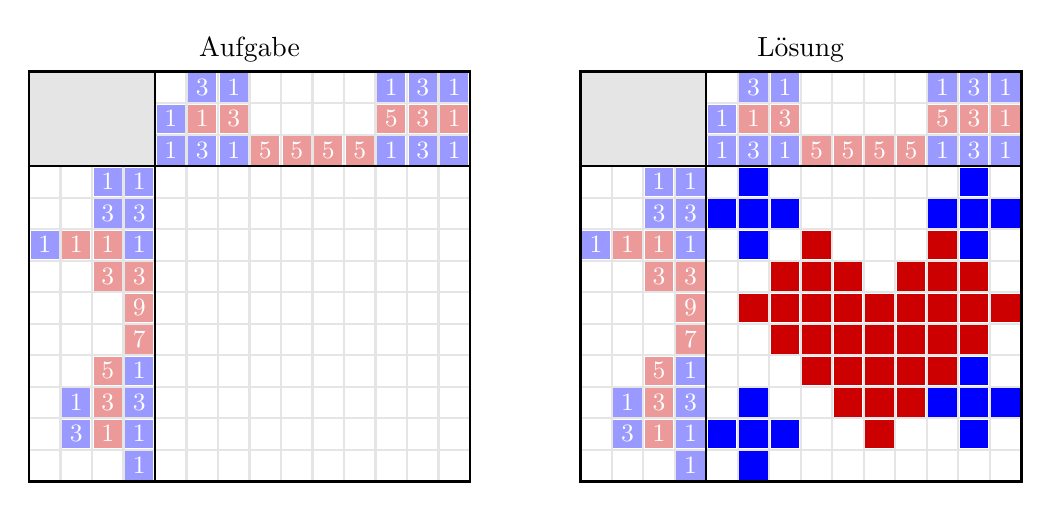
\begin{tikzpicture}[>=latex,thick]
\begin{scope}[xshift=-3.5cm]
\node at ({3*\h},{3*\h}) [above] {Aufgabe};
\rahmen
\end{scope}
\begin{scope}[xshift=3.5cm]
\node at ({3*\h},{3*\h}) [above] {Lösung};
\rahmen
          \b{1}{0}                                                    \b{8}{0}
\b{0}{-1} \b{1}{-1} \b{2}{-1}                               \b{7}{-1} \b{8}{-1} \b{9}{-1}
          \b{1}{-2}           \r{3}{-2}                     \r{7}{-2} \b{8}{-2}
                    \r{2}{-3} \r{3}{-3} \r{4}{-3}           \r{6}{-3} \r{7}{-3} \r{8}{-3}
          \r{1}{-4} \r{2}{-4} \r{3}{-4} \r{4}{-4} \r{5}{-4} \r{6}{-4} \r{7}{-4} \r{8}{-4} \r{9}{-4}
                    \r{2}{-5} \r{3}{-5} \r{4}{-5} \r{5}{-5} \r{6}{-5} \r{7}{-5} \r{8}{-5}
          \b{1}{-7}           \r{3}{-6} \r{4}{-6} \r{5}{-6} \r{6}{-6} \r{7}{-6} \b{8}{-6}
\b{0}{-8} \b{1}{-8} \b{2}{-8}           \r{4}{-7} \r{5}{-7} \r{6}{-7} \b{7}{-7} \b{8}{-7} \b{9}{-7}
          \b{1}{-9}                               \r{5}{-8}                     \b{8}{-8}
\end{scope}
\end{tikzpicture}
\end{center}
Die Vorgabe blau 1, rot 3, blau 3 in der drittuntersten Zeile bedeutet,
dass in dieser Zeile zunächst ein einzelnes blaues Feld vorkommen muss,
dann drei benachbarte rote Felder gefolgt von 3 benachbarten blauen Feldern.

Das Problem {\em NONOGRAM} ist also die Aufgabe, zu entscheiden, ob
ein Nonogramm-Rätsel überhaupt lösbar ist.
\begin{teilaufgaben}
\item Ist {\em NONOGRAM} entscheidbar?
\item Kann eine nichtdeterministische Turing-Maschine in polynomieller Zeit
entscheiden, ob ein Nonogram gelöst werden kann?
\end{teilaufgaben}

\thema{polynomieller Verifizierer}
\thema{Entscheidbarkeit}
\thema{NP}

\begin{loesung}
\begin{teilaufgaben}
\item
Wenn $c$ verschiedene Farben gewählt werden können, dann gibt es für
jedes der $nm$ Felder $c+1$ Wahlmöglichkeiten. 
Das Feld kann daher auf $(c+1)^{nm}$ verschiedene Arten ausgfüllt
werden.
Indem man alle diese Möglichkeiten durchprobiert kann man immer entscheiden,
ob die Aufgabe lösbar ist.
Das Problem ist also entscheidbar.
\item
Wir brauchen einen polynomiellen Entscheider.
Als Lösungszertifikat verlangen wir die Belegung der Felder mit Farben.
folgendes muss überprüft werden:
\begin{center}
\begin{tabular}{lrrr}
Was&Anzahl&Aufwand&Total\\
\hline
\begin{minipage}[t]{0.6\hsize}
\strut
Jede Zeile durchlesen und überrüfen, ob die vorgeschriebenen Lauflängen
jeder Farbe vorliegen.\strut
\end{minipage}&$n$&$O(m)$&$O(mn)$\\
\begin{minipage}[t]{0.6\hsize}
\strut
Jede Spalte durchlesen und überrüfen, ob die vorgeschriebenen Lauflängen
jeder Farbe vorliegen.\strut
\end{minipage}&$m$&$O(n)$&$O(mn)$\\
\hline
\strut
Total&&&$O(mn)$
\end{tabular}
\end{center}
Dies zeigt, dass die Lösung in polynomieller Zeit in der Problemgrösse
$N=mn$ verifiziert werden kann. 
Es folgt, dass das Problem
{\em NOMOGRAM} in NP ist.
\qedhere
\end{teilaufgaben}
\end{loesung}

\begin{diskussion}
Nobuhisa Ueda und Tadaaki Nagao haben 1996 bewiesen, dass
{\em NONOGRAM} NP-vollständig ist:
{\em NP-completeness Results for NONOGRAM via Parsimonious Reductions},
Technical Report,
Departement of Computer Science,
Tokyo Institue of Technology, doi:10.1.1.57.5277
\end{diskussion}

\begin{bewertung}
Entscheidbarkeit ({\bf E}) 1 Punkt,
Verifizierer ({\bf V}) 1 Punkt,
Zertifikat ({\bf Z}) 1 Punkt,
Verifikationsalgorithmus ({\bf A}) 2 Punkte,
Nachweis, dass Aufwand polynomiell ist ({\bf P}) 1 Punkte.
\end{bewertung}

